\documentclass[a4paper,11pt]{article}

\usepackage{latexsym}
\usepackage{graphicx}
\usepackage{float}
\usepackage[margin=2cm]{geometry}
\usepackage{lscape}
\usepackage{underscore}
\usepackage{amsmath}
\usepackage{blindtext}
\usepackage{listings}
\usepackage{xcolor}
\usepackage{mathtools}

\usepackage[all]{nowidow}

\usepackage[LY1]{fontenc}
\usepackage[utf8x]{inputenc}
\usepackage{polski}
\usepackage[lf,enc=t1]{berenis}

\DeclareTextCompositeCommand{\k}{LY1}{a}
  {\oalign{a\crcr\noalign{\kern-.27ex}\hidewidth\char7}}


\usepackage{listings}
\usepackage{color}

\definecolor{mygreen}{rgb}{0,0.6,0}
\definecolor{mygray}{rgb}{0.5,0.5,0.5}
\definecolor{mymauve}{rgb}{0.58,0,0.82}

\lstset{ %
  backgroundcolor=\color{white},   % choose the background color; you must add \usepackage{color} or \usepackage{xcolor}; should come as last argument
  basicstyle=\footnotesize,        % the size of the fonts that are used for the code
  breakatwhitespace=false,         % sets if automatic breaks should only happen at whitespace
  breaklines=true,                 % sets automatic line breaking
  captionpos=b,                    % sets the caption-position to bottom
  commentstyle=\color{mygreen},    % comment style
  deletekeywords={...},            % if you want to delete keywords from the given language
  escapeinside={\%*}{*)},          % if you want to add LaTeX within your code
  extendedchars=true,              % lets you use non-ASCII characters; for 8-bits encodings only, does not work with UTF-8
  frame=single,	                   % adds a frame around the code
  keepspaces=true,                 % keeps spaces in text, useful for keeping indentation of code (possibly needs columns=flexible)
  keywordstyle=\color{blue},       % keyword style
  language=Java,                 % the language of the code
  morekeywords={*,...},            % if you want to add more keywords to the set
  numbers=left,                    % where to put the line-numbers; possible values are (none, left, right)
  numbersep=5pt,                   % how far the line-numbers are from the code
  numberstyle=\tiny\color{mygray}, % the style that is used for the line-numbers
  rulecolor=\color{black},         % if not set, the frame-color may be changed on line-breaks within not-black text (e.g. comments (green here))
  showspaces=false,                % show spaces everywhere adding particular underscores; it overrides 'showstringspaces'
  showstringspaces=false,          % underline spaces within strings only
  showtabs=false,                  % show tabs within strings adding particular underscores
  stepnumber=2,                    % the step between two line-numbers. If it's 1, each line will be numbered
  stringstyle=\color{mymauve},     % string literal style
  tabsize=2,	                   % sets default tabsize to 2 spaces
  title=\lstname                   % show the filename of files included with \lstinputlisting; also try caption instead of title
}



\begin{document}
\begin{titlepage}


\newcommand{\HRule}{\rule{\linewidth}{0.5mm}}
\center

\textsc{\LARGE Politechnika Wrocławska}\\[1.5cm]
\textsc{\LARGE Projektowanie efektywnych algorytmów}\\[0.5cm]

\HRule \\[0.5cm]
{ \huge \bfseries Projekt nr 3: \\[0.3cm]Implementacja i analiza efektywności algorytmu genetycznego (ewolucyjnego) dla problemu komiwojażera  }\\[0.5cm] 
\HRule \\[1.5cm]

\begin{flushleft} \large
 
\emph{Autor:}\\
 
Bartosz  \textsc{Pogoda} 225988 \\
 
\end{flushleft}
%\end{minipage}
 
%\begin{minipage}{0.4\textwidth}
\begin{flushright} \large
 
\emph{Prowadzący:} \\
dr inż. Jarosław \textsc{Mierzwa} 
 
\end{flushright}
%\end{minipage}\\[4cm]
 
\vfill
{\large 8 stycznia 2018}\\[3cm] 
 
 
\end{titlepage}

\tableofcontents
\newpage

\section{Wstęp teoretyczny}

\subsection{Opis problemu}

Problem komiwojażera definiowany jest dla grafów pełnych. Wierzchołki grafu nazywane są miastami,
a krawędziom przypisane są wartości reprezentujące odległości między nimi. Problem polega na
odnalezieniu najkrótszej ścieżki, takiej aby odwiedzić każde miasto dokładnie raz i wrócić do punktu
wyjścia. \newline

Wiele problemów, występujących w sektorach takich jak transport oraz logistyka można sprowadzić
do problemu komiwojażera. Zastosowanie efektywnych algorytmów rozwiązujących ten problem nie
rzadko prowadzi do redukcji kosztów i optymalizacji pewnych rzeczywistych procesów. Przykładową
aplikacją mogło by być wyznaczenie optymalnej trasy dla autobusu szkolnego, tak aby odwiedził
wszystkie przystanki z dziećmi w jak najkrótszym okresie czasu. Wierzchołkami grafu byłyby
poszczególne przystanki, a wartościami na krawędziach szacunkowy czas przemieszczenia się autobusu
między przystankami. Warto tutaj zauważyć, że czas przemieszczania się z przystanku A do B, może
różnić się od czasu przemieszczenia z B do A. Różnice te są uwzględnione w asymetrycznym problemie
komiwojażera, który zostanie poddany analizie w tym sprawozdaniu.

\subsection{Opis algorytmu}

Algorytmy genetyczne (ewolucyjne) opierają się założeniach teorii ewolucji Darwina. Procesy dotyczące selekcji naturalnej występujące w rzeczywistym środowisku są symulowane w celu rozwiązania problemów optymalizacyjnych. Podstawową zasadą, która sugeruje skuteczność takich algorytmów jest fakt, że z biegiem czasu (w wyniku ewolucji oraz selekcji naturalnej) populacja staję się coraz lepiej przystosowana do środowiska, w którym żyje, o ile warunki środowiska diametralnie się nie zmieniają - co zazwyczaj nie ma miejsca w przypadku problemów, dla których tworzymy takie algorytmy. 

\subsection{Kroki algorytmu}

Podstawowy algorytm genetyczny składa się z kroków opisanych poniżej. Etapy procesu (1.3.2 - 1.3.5) są powtarzane wielokrotnie aż do osiągnięcia kryterium stopu.

\subsubsection{Inicjalizacja}

Zostaje utworzona początkowa populacja, o określonej wielkości. Podczas inicjaizacji w obrębie projektu jedna ścieżka jest znajdowana za pomoca algorytmu zachłannego, a reszta generowana jest w sposób losowy.

\subsubsection{Ewaluacja - wyznaczenie przystosowania}

Wyznaczane są wartości przystosowania jednostek populacji. W tym celu definiuje się specjalną funkcję przystosowania (funkcja FIT), która mierzy jak "dobra" jest dana jednostka. Dla problemu komiwojażera wartość przystosowania jednostki-ścieżki określa się jako odwrotność jej długości.

W obrębie projektu osobnik najlepiej przystosowany jest bezpośrednio umieszczany w następnej generacji. Interpretacją biologiczną mogłoby tutaj być umieszczenie dobrze przystosowanego osobnika w inkubatorze na czas jednej generacji, w celu zapobiegnięcia modyfikacji jego materiału genetycznego.

\subsubsection{Selekcja}

W tym kroku następuje wybór z populacji jednostek, które zostaną rodzicami dla kolejnej generacji. Jedną z metod wyboru jest metoda turniejowa - organizowane są turnieje o określonej wielkości, do których dobiera się uczestników w sposób losowy. Turniej wygrywa najlepiej przystosowany osobnik (maksymalna wartość funkcji FIT). Warto tutaj zaznaczyć, że dobór wielkośći turnieju jest istotny. Małe turnieje zwiększają "dywersyfikację" przestrzeni rozwiązań, ponieważ zwiększają szansę jednostek "słabych", które jednak w wyniku krzyżowania mogą dać nowe, potencjalnie lepsze rozwiązania. Duże turnieje znacznie fawozyrują jednostki lepiej przystosowane, co może prowadzić do osiągnięcia minimum lokalnego. 

\subsubsection{Krzyżowanie}

Osobniki wybrane w fazie selekcji są krzyżowane w celu wymieszania ich cech. W wyniku krzyżowania powstaje dziecko, które w idealnym przypadku odziedziczyłoby najlepsze cechy obojga rodziców. Definiowane jest prawdopodobieństwo z jakim odbędzie się krzyżowanie.

\begin{itemize}
\item Krzyżowanie PMX

Operator PMX (Partially-Matched Crossover) gwarantuje brak powtórzeń genów (numerów miast) w powstałym chromosomie (w powstałej ścieżce). Podczas operacji krzyżowania w pierwszej kolejności losowany jest pewien zakres kolejnych pozycji ścieżki. Następnie miasta pierwszego rodzica objęte tym zakresem są kopiowane bezpośrednio do dziecka (odpowiadające sobie pozycje objęte zakresem). W nastepnej kolejności miasta drugiego rodzica objęte zakresem, które jeszcze nie są uwzględnione w dziecku, są kopiowane do dziecka. W tym kroku pozycje wyznaczane są na podstawie poszukiwań pozycji, którą zajmuje odpowiadające (ta sama pozycja) miasto rodzica pierwszego w ścieżce rodzica drugiego. Taka procedura gwarantuje, że zostaną zapełnione miejsca, którym odpowiadały miasta już uwzględnione w ścieżce. Ostatecznie miasta rodzica drugiego nieobjęte zakresem są przepisywane na odpowiadące pozycje dziecka.

Przykład:
pierwszyRodzic: [0 1 \textbf{2 3} 4 0], drugiRodzic: [0 2 \textbf{3 1} 4 0], zakres(2,3)
\newline dziecko:
\newline 1. Miasto poczatkowe zostaje przepisane-  [\textbf{0} _ _ _ _ \textbf{0}]
\newline 2. Geny pierwszego rodzica zostają przepisane-  [0 _  \textbf{2 3} _ 0]
\newline 3. Miasto w zakresie drugiego rodzica "1" nie wystepuje w dziecku. Miastu temu w pierwszym rodzicu odpowiada miasto "3". Miasto to w drugim rodzicu znajduje się w zakresie, a więc krok jest powtarzany. Miastu "3" w pierwszym rodzicu odpowiada miasto "2". Miasto to jest na pozycji 1 w drugim dziecku. Pozycja ta nie znajduje się w zakresie, a więc zostaje ona wybrana jako pozycja dla miasta "1". 
\newline A więc: [0 \textbf{1}  2 3 _ 0]
\newline 4. Pozostałe miasta uzupełniane są odpowiadającymi miastami w rodzicu drugim:  [0 1 2 3  \textbf{4} 0]

\end{itemize}


\subsubsection{Mutacja}

Nowo powstała populacja złożona z dzieci oraz osobników, którzy nie zostali poddani krzyżowaniu (tak zadecydował rzut na prawdopodobieństwo krzyżowania), zostaje poddania mutacji, również z określonym prawdopodobieństwem. Zjawisko mutacji pozwala na zwiększenie dywersyfikacji. W wyniku mutacji mogą powstać pożądane cechy, których nie udałoby sie uzyskać za pomocą krzyżowania osobników.

\begin{itemize}
\item Mutacja Swap

Losowane są dwie różne pozycje ścieżki, a następnie odpowiadające im miasta zostają wymienione między sobą. 
Przykład:
[0 1 2 3 4 5 0]  -- Swap(1,4) --> [0 4 2 3 1 5 0]

\item Mutacja Invert

Losowany jest zakres pozycji ścieżki, a następnie występujące w tym zakresie miasta zostają odwrocone kolejnością.
Przykład:
[0 1 2 3 4 5 0]  -- Invert(1,4) --> [0 4 3 2 1 5 0]

\end{itemize}

\newpage
\section{Implementacja algorytmu, opis istotnych klas}
\subsection{Instancja}

Klasa reprezentująca instancję problemu. Przechowuje informacje o krawędziach w postaci macierzy sąsiedztwa.

\subsection{CrossoverOperator}

Interfejs CrossoverOperator deklaruję metodę crossover, która służy do krzyżowania dwóch osobników. Implementacja PMXCrossoverOperator realizuje metodę PMX opisaną w 1.3.4. Klasa pomocnicza MatchingSectionBounds służy do przechowywania wylosowanego zakresu dla krzyżowania.


\begin{figure}[H]
\centering
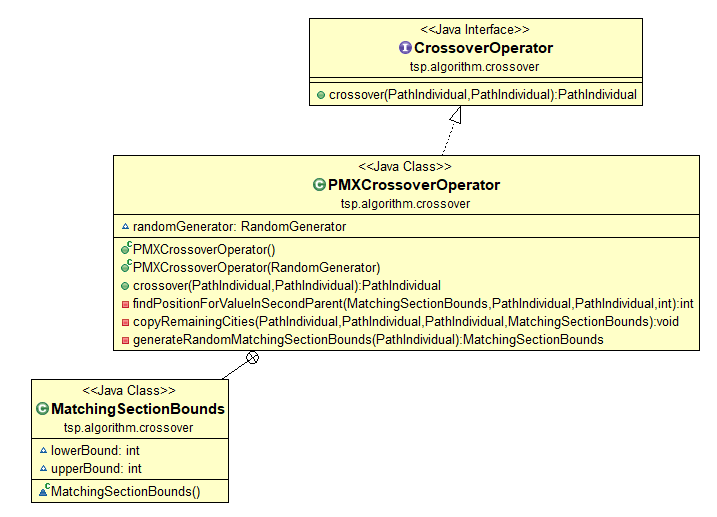
\includegraphics[height=10cm]{crossover.PNG}
\caption{Pakiet: crossover}
\end{figure}


\subsection{PathIndividual}

PathIndividual definiuje osobnika - rozwiązanie problemu komiwojażera. Klasa PathIndividualGenerator potrafi wygenerować losową ścieżkę, jak również, ścieżkę zachłanną.

\begin{figure}[H]
\centering
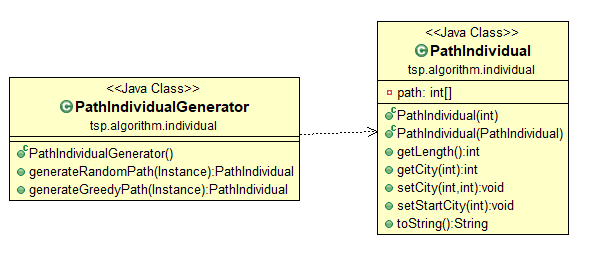
\includegraphics[height=5cm]{pathIndividual.PNG}
\caption{Pakiet: individual}
\end{figure}

\subsection{MutationOperator}

Interfejs MutationOperator jest implementowany przez dwa konkretne rodzaje mutacji - SwapMutationOperator oraz InvertMutationOperator. Zasada działania poszczególnych mutacji została opisana w podpunkcie 1.3.5.

\begin{figure}[H]
\centering
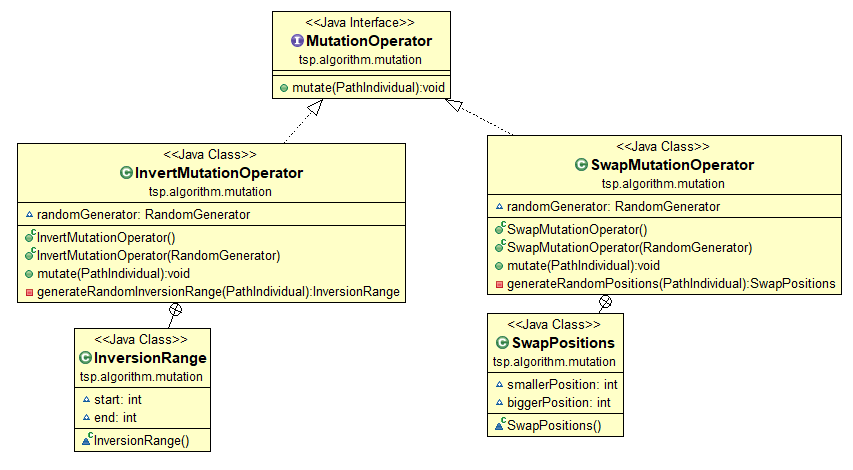
\includegraphics[height=10cm]{mutation.PNG}
\caption{Pakiet: mutation}
\end{figure}

\subsection{PathPopulation}

Klasa PathPopulation reprezentuje populację w algorytmie, a więc agreguje osobników (PathIndividual). Klasa deklaruje również operacje znalezienia najlepiej przystosowanego osobnika spośród wystepujących w populacji oraz metode statyczną generującą startową populację.

\begin{figure}[H]
\centering
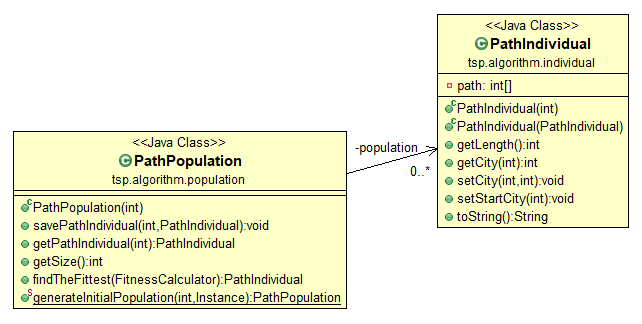
\includegraphics[height=7cm]{population.PNG}
\caption{Pakiet: population}
\end{figure}

\subsection{TournamentChooser, FitnessCalculator }

TournamentChooser służy do wyboru osobników z populacji metodą turniejową. FitnessCalculator udostępnia metodę calculateFitness służącą do wyznaczenia wartości przystosowania konkretnego osobnika.

\begin{figure}[H]
\centering
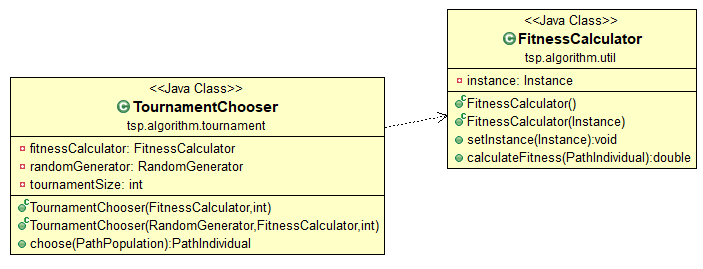
\includegraphics[height=6cm]{util.PNG}
\caption{Pakiety: tournament, util}
\end{figure}

\subsection{Algorithm}

Klasa Algorithm zarządza całym algorytmem (procesem ewolucji). AlgorithmBuilder jest klasą pomoczniczą, służącą do wygodnego tworzenia instancji klasy Algorithm podając jego konfigurację oraz inne parametry (wzorzec projektowy Builder). Klasa AlgorithmTerminator realizuje kryterium stopu w postaci czasu wykonywania się algorytmu. Klasa BestDistanceSampler zajmuje się próbkowaniem aktualnie najlepszej wartości ścieżki oraz zapisem jej do pliku / wypisaniem na ekran.

\begin{figure}[H]
\centering
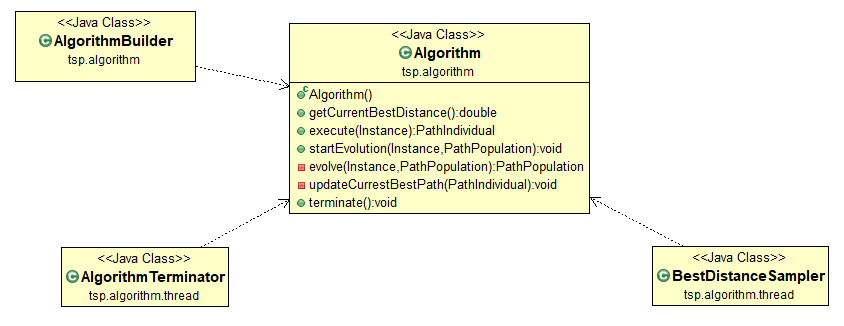
\includegraphics[height=7cm]{algorithm.PNG}
\caption{Pakiet: algorithm}
\end{figure}

\newpage
\section{Wyniki badań}

Po zaimplementowaniu algorytmu oraz klas pomoczniczych zostały przeprowadzone testy jakościowe.

\subsection{Parametry}

\begin{itemize}
\item Badania przeprowadzono na instancjach eil101.tsp, rbg403.atsp oraz d1291.tsp
\item Algorytm został zbadany dla następujących wielkości populacji: 1/10*N, 1/2*N, N \newline (gdzie N jest wielkością instancji)
\item Dla powyższych wielkości populacji zostały zbadane mutacje Swap oraz Invert.
\item Dla najlepszej wielkości populacji oraz rodzaju mutacji został zbadany wpływ współczynnika mutacji. Wartości: 0.02, 0.05, 0.1
\item Ograniczenie czasowe algorytmu zostało ustawione na 6 minut.
\end{itemize}

\newpage
\subsection{Instancja - eil101.tsp}

Optymalna długość ścieżki: 629
\newline Najlepsza znaleziona długość ścieżki: 675

\subsubsection{Tabele zbiorcze}


\begin{figure}[H]
\centering
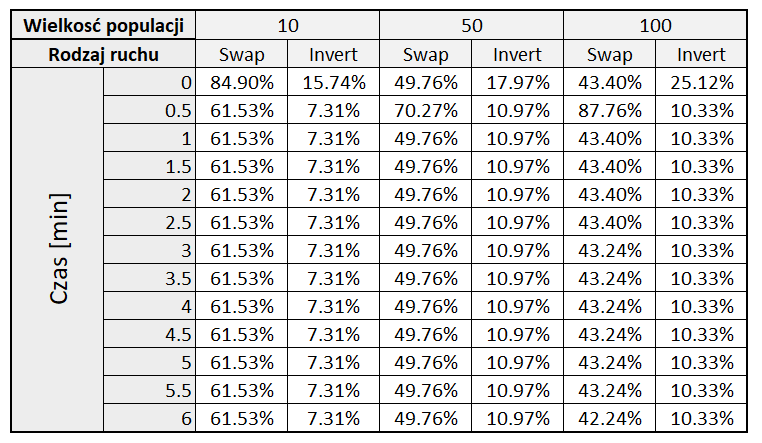
\includegraphics[height=9cm]{t1.PNG}
\caption{Zależnośc błędu względnego od czasu dla różnych kombinacji parametrów (eil101.tsp)}
\end{figure}

\begin{figure}[H]
\centering
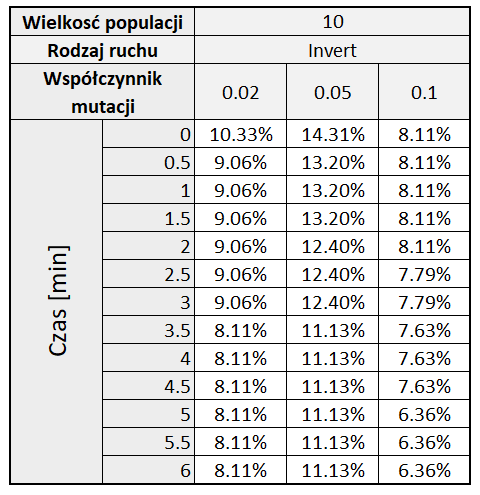
\includegraphics[height=9cm]{t4.PNG}
\caption{Zależnośc błędu względnego od czasu dla różnych współczynników mutacji oraz najlepszej kombinacji z poprzedniej tabeli (eil101.tsp)}
\end{figure}


\newpage
\subsubsection{Wykresy}

\begin{figure}[H]
\centering
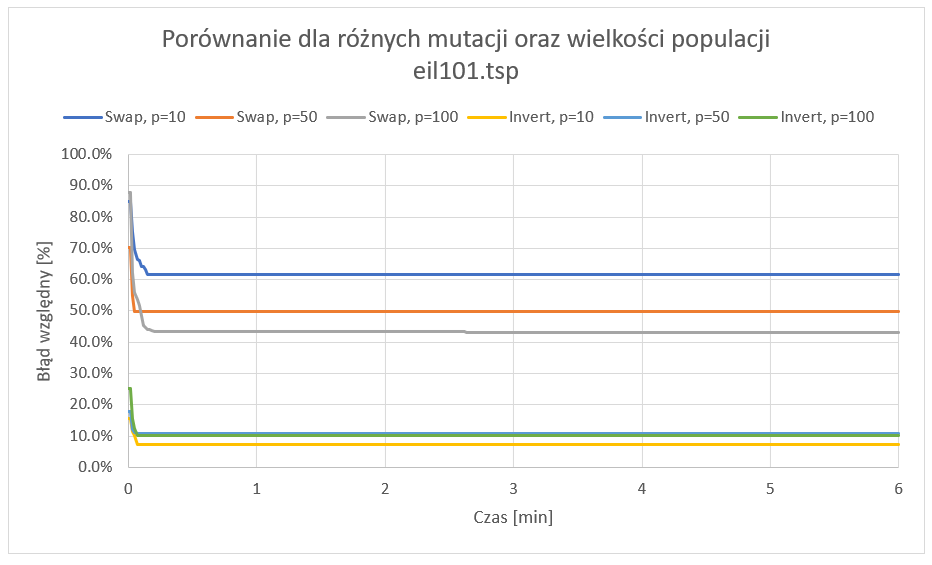
\includegraphics[height=10cm]{w1.PNG}
\caption{Zależnośc błędu względnego od czasu dla różnych kombinacji parametrów (eil101.tsp)}
\end{figure}

\begin{figure}[H]
\centering
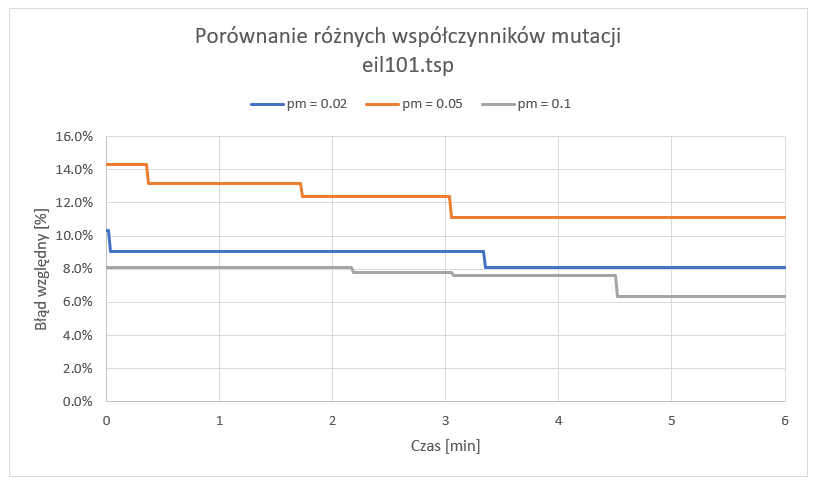
\includegraphics[height=10cm]{w4.PNG}
\caption{Zależnośc błędu względnego od czasu dla różnych współczynników mutacji - pm (eil101.tsp)}
\end{figure}

\newpage
\subsection{Instancja - rbg403.atsp}

Optymalna długość ścieżki: 2465
\newline Najlepsza znaleziona długość ścieżki: 2755

\subsubsection{Tabele zbiorcze}

\begin{figure}[H]
\centering
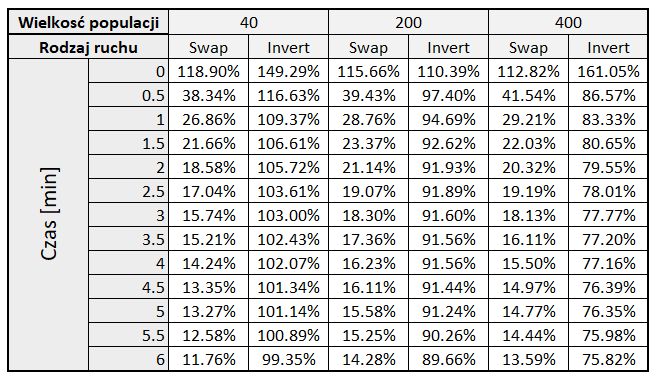
\includegraphics[height=9cm]{t2.PNG}
\caption{Zależnośc błędu względnego od czasu dla różnych kombinacji parametrów (rbg403.atsp)}
\end{figure}

\begin{figure}[H]
\centering
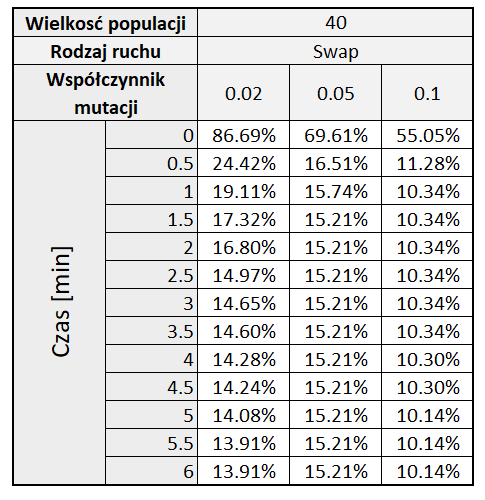
\includegraphics[height=9cm]{t5.PNG}
\caption{Zależnośc błędu względnego od czasu dla różnych współczynników mutacji oraz najlepszej kombinacji z poprzedniej tabeli (rbg403.atsp)}
\end{figure}

\newpage
\subsubsection{Wykresy}

\begin{figure}[H]
\centering
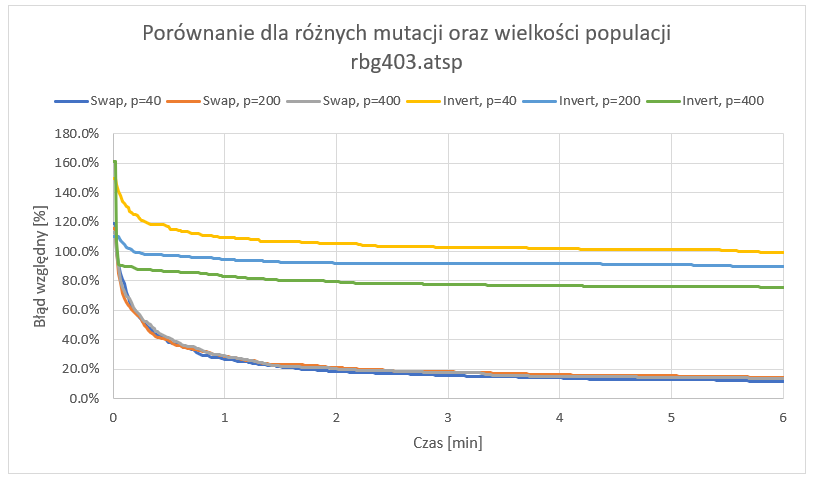
\includegraphics[height=10cm]{w2.PNG}
\caption{Zależnośc błędu względnego od czasu dla różnych kombinacji parametrów (rbg403.atsp)}
\end{figure}

\begin{figure}[H]
\centering
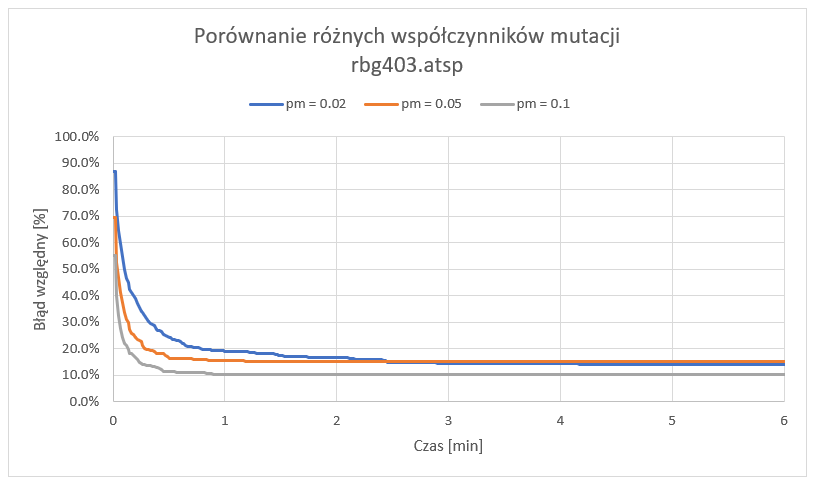
\includegraphics[height=10cm]{w5.PNG}
\caption{Zależnośc błędu względnego od czasu dla różnych współczynników mutacji - pm (rbg403.atsp)}
\end{figure}



\newpage
\subsection{Instancja - d1291.tsp}

Optymalna długość ścieżki: 50801
\newline Najlepsza znaleziona długość ścieżki: 234287

\subsubsection{Tabele zbiorcze}

\begin{figure}[H]
\centering
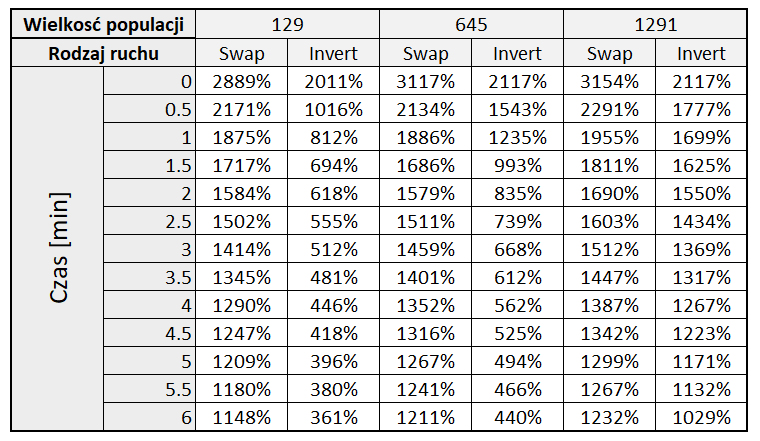
\includegraphics[height=9cm]{t3.PNG}
\caption{Zależnośc błędu względnego od czasu dla różnych kombinacji parametrów (d1291.tsp)}
\end{figure}

\begin{figure}[H]
\centering
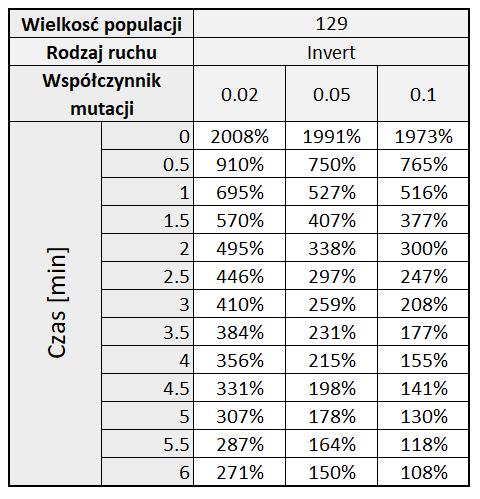
\includegraphics[height=9cm]{t6.PNG}
\caption{Zależnośc błędu względnego od czasu dla różnych współczynników mutacji oraz najlepszej kombinacji z poprzedniej tabeli (d1291.tsp)}
\end{figure}
\newpage
\subsubsection{Wykresy}

\begin{figure}[H]
\centering
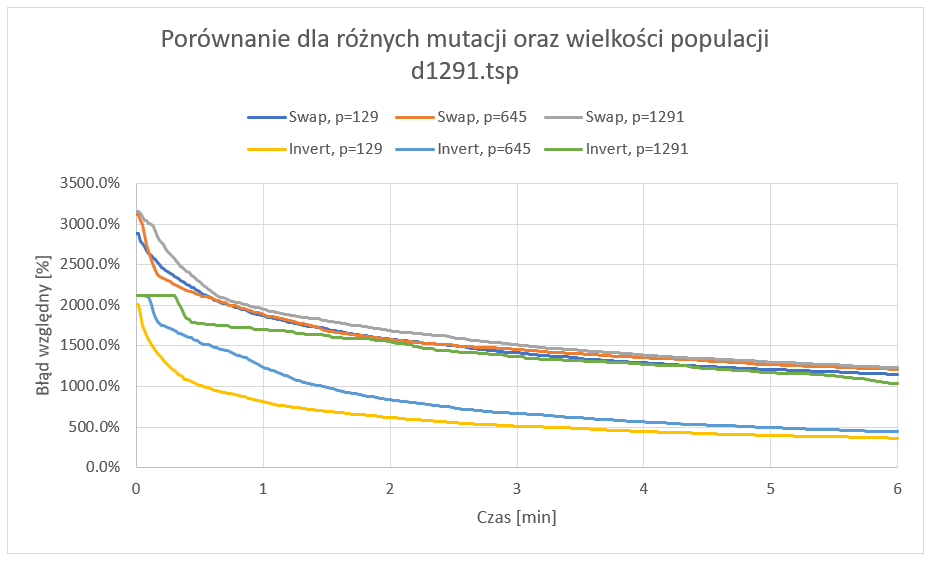
\includegraphics[height=10cm]{w3.PNG}
\caption{Zależnośc błędu względnego od czasu dla różnych kombinacji parametrów (d1291.tsp)}
\end{figure}

\begin{figure}[H]
\centering
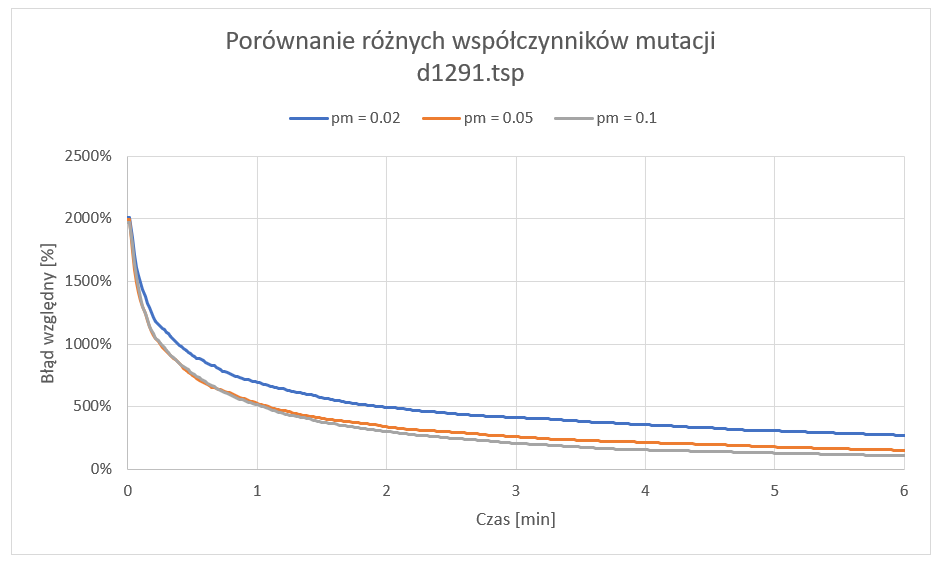
\includegraphics[height=10cm]{w6.PNG}
\caption{Zależnośc błędu względnego od czasu dla różnych współczynników mutacji - pm (d1291.tsp)}
\end{figure}


\newpage
\section{Podsumowanie, wnioski}

Zaimplementowany algorytm skutecznie radził sobie z znajdywaniem rozwiązań bliskich optymalnemu w krótkim czasie, mimo dużych rozmiarów instancji. 

\begin{itemize}
\item Algorytm jest bardzo wrażliwy na konfigurację. Dobór parametrów do konkretnej instancji problemu jest kluczowy w celu uzyskania dobrych wyników.
\item Mutacja typu Invert sprawdza się lepiej niż typu Swap dla problemu symetrycznego.
\item Mutacja typu Invert sprawdza się gorzej niż typu Swap dla problemu asymetrycznego.
\item Dla każdej z instancji ustawienie parametru mutacji na najwyższą badaną wartośc (0.1) dało najlepsze rezultaty.
\item Najszybszy wzrost jakości rozwiązań występuje w początkowej fazie działania algorytmu genetycznego (duże nachylenie w początkowej części wykresów)
\item Okres szybkiego wzrostu jakości rozwiązań jest proporcjonalny do wielkości instancji. Dla instancji wielkości 101 trwał niecałe 10s, dla instancji wielkości 1291-  minutę.
\item Dla małych instancji na wzrost jakości rozwiązań może mieć duży wpływ skonfigurowana dywersyfikacja, która w przypadku tego algorytmu może być zwiększona za pomocą parametru mutacji oraz wielkości turniejów.
\item Im mniejsze turnieje tym większa dywersyfikacja - dopuszczanych jest więcej słabszych rozwiązań, które dla dużych turniejów są wypierane przez rozwiązania najlepsze w populacji. Dywersyfikacja może prowadzić do lepszych rezultatów końcowych.

\end{itemize}















\end{document}